\section{Scelte implementative}
\label{cap:implementation-choices}

\subsection{Codice templatizzato}

\subsection{Rappresentazione del grafo}

Le due possibilità standard per rappresentare un grafo sono 
\begin{itemize}
	\item \textbf{Matrici di adiacenza}
	\item \textbf{Liste di adiacenza}
\end{itemize}

Tuttavia in questa implementazione abbiamo scelto di utilizzare una \textbf{"mappa di adiacenza"} affiancata con un set non ordinato per migliorare le complessità temporali di alcune operazioni fondamentali sul grafo, a scapito di un aumento della complessità spaziale. Una prima panoramica della classe è possibile osservarla con il diagramma di classe in figura~\ref{fig:AdjMapGraph Class} dove vengono riportati gli attributi e i metodi offerti dalla classe.

\begin{figure}[h]
	\caption{Diagramma di classe per AdjListGraph}
	\centering
	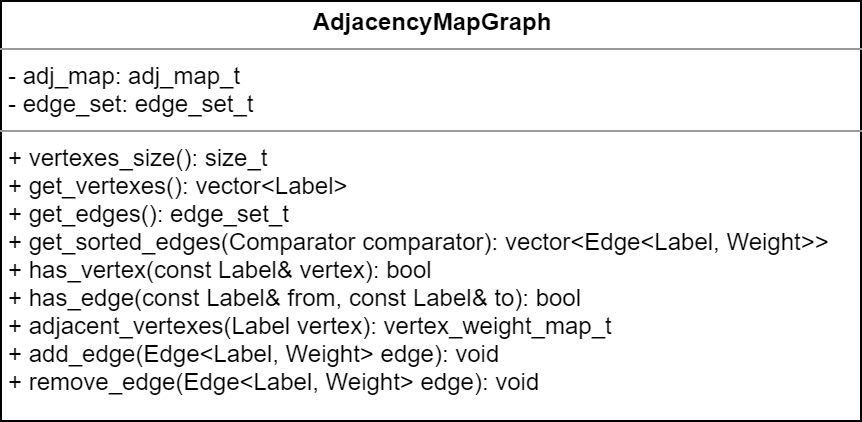
\includegraphics[width=0.7\textwidth]{./images/AdjancencyMapGrapClass.png}
	\label{fig:AdjMapGraph Class}
\end{figure}

Nella figura~\ref{fig:AdjMapGraph Abstract} è riportata la trasformazione di un grafo di esempio nella relativa mappa di adiacenza che abbiamo pensato. Come è possibile notare questa mappa di adiacenza è composta da una prima mappa che elenca tutti i vertici del grafo (adj\_map\_t) e a seguire nel valore di ogni entry viene inserita una nuova mappa (vertex\_weight\_map\_t) che rappresenta gli archi del grafo: vengono elencati dunque tutti i nodi adiacenti al vertice dato con il relativo peso dell'arco. In questo modo è possibile avere tutte le operazioni di inserimento, ricerca, cancellazione e update in tempo costante, a discapito di una complessità spaziale più elevata. 

\begin{figure}[h]
	\caption{Rappresentazione della mappa di adiacenza}
	\centering
	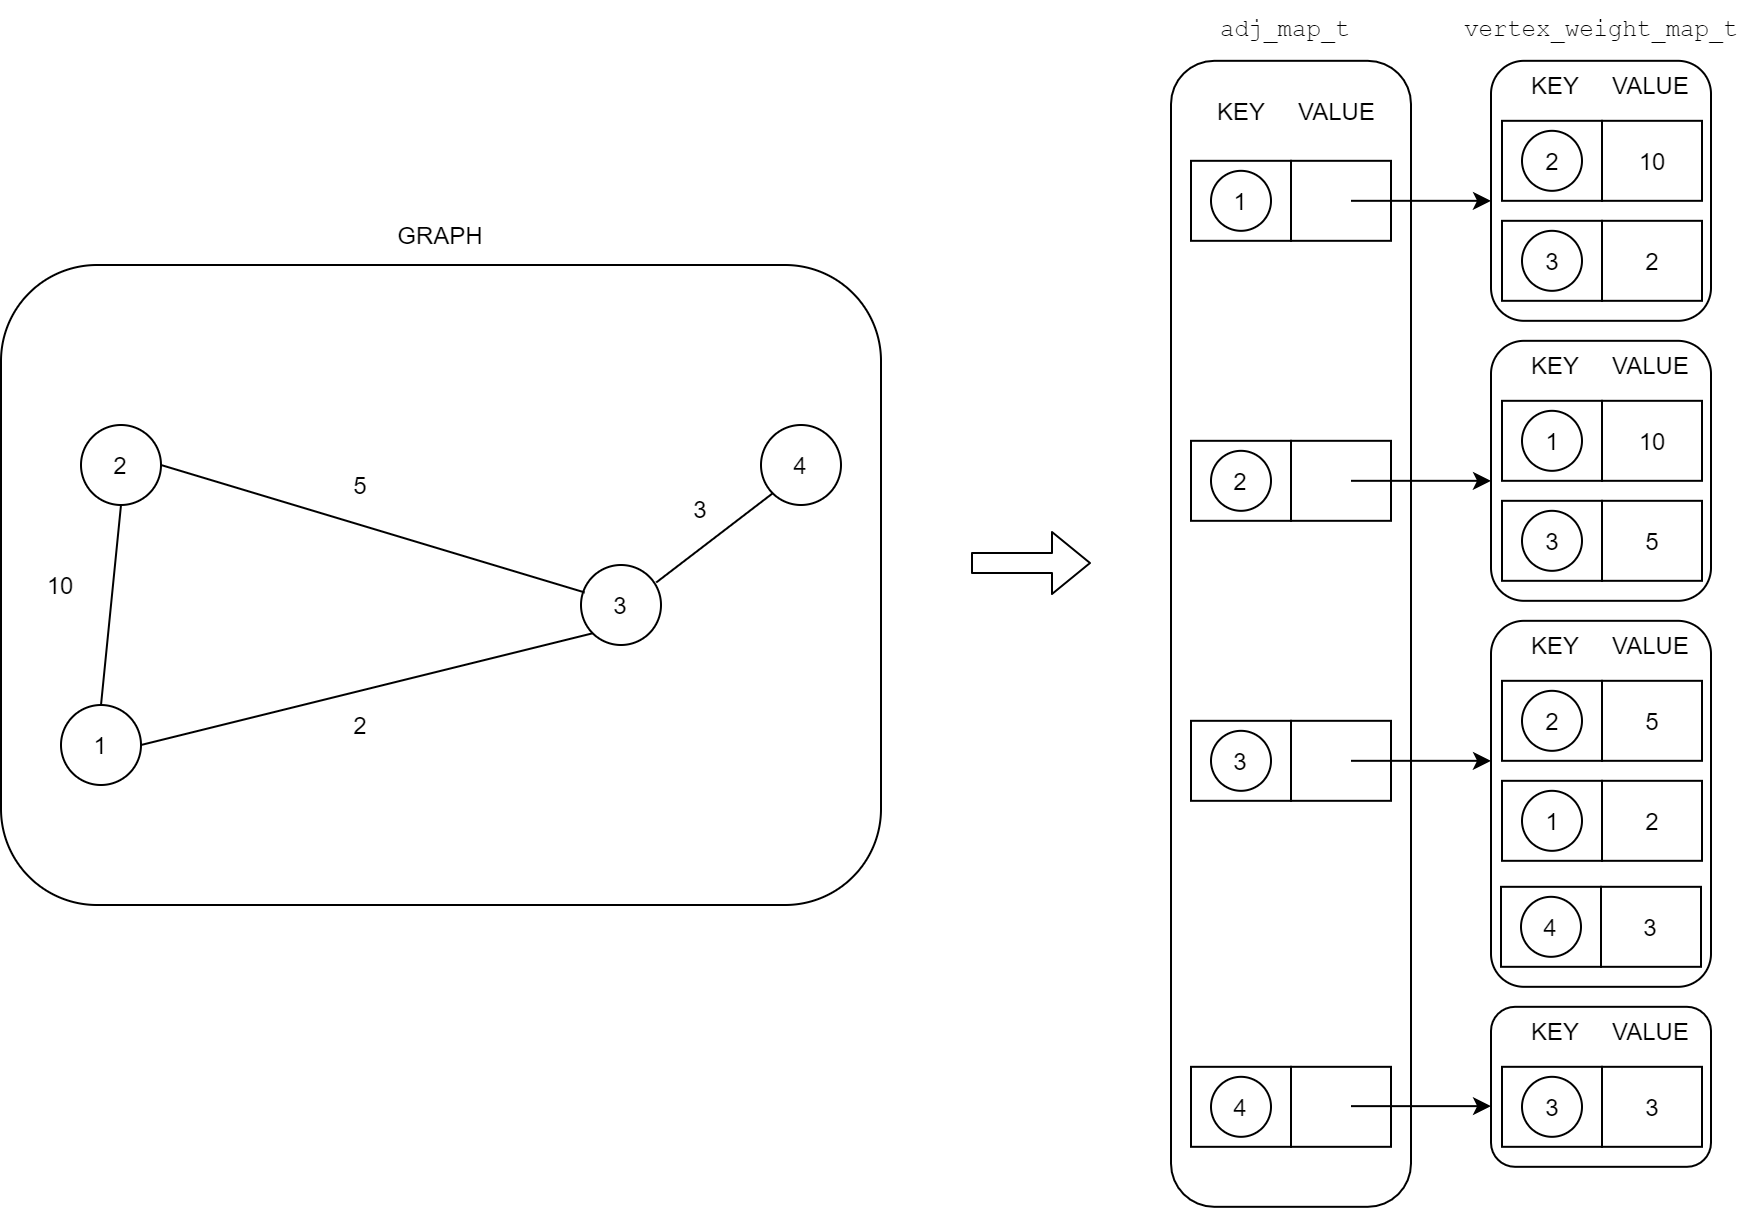
\includegraphics[width=0.7\textwidth]{./images/AdjMapGraphAbstract.png}
	\label{fig:AdjMapGraph Abstract}
\end{figure}

Nonostante la mappa di adiacenza sarebbe già stata sufficiente per salvare tutte le informazioni necessarie alla rappresentazione di un grafo, in alcune operazioni risulta essere lenta. L'esempio di operazione che ci ha spinto ad inserire una nuova struttura dati (unordered\_set in questo caso) è il metodo per ritornare tutti gli archi di un grafo in quanto tale metodo se implementato avendo a disposizione la sola mappa di adiacenza prevederebbe in maniera semplice la scansione dell'intera mappa di adiacenza, con l'inserimento degli archi via via che si incontra un nuovo vertice. Tale semplice implementazione però porterebbe alla creazione di un vettore in cui se sussiste un arco tra un vertice 2 e un vertice 3 (come nell'esempio in figura~\ref{fig:AdjMapGraph Abstract}), al vettore verrebbe aggiunto sia l'arco 2 $\rightarrow$ 3 che 3 $\rightarrow$ 2. \\

Le cose si complicano maggiormente infatti se si restringe la richiesta di non restituire gli archi doppi come abbiamo già osservato. A tale proposito si potrebbe ricercare l'eventuale presenza di tali archi doppi ed eliminarli di conseguenza, ma il tutto richiederebbe maggiori operazioni e dunque un maggior complessità temporale.\\

Per tali ragioni è stato deciso di affiancare alla mappa di adiacenza, un'apposita struttura dati che permettesse di tenere traccia degli archi e di avere tempi di esecuzione costanti per le operazioni di aggiunta, rimozione e ricerca. Così facendo è possibile garantire che l'operazione di restituzione degli archi singoli di un grafo abbia tempo O(m) se si richiede di restituire un vettore, o addirittura O(1) se si richiede la restituzione di un puntatore a tale struttura.
E' stato scelto dunque di utilizzare come struttura dati da affiancare unordered\_set perché oltre ad avere le caratteristiche richieste, se appositamente configurata permette di garantire l'assenza di archi doppi, compresi quelli visti nell'esempio precedente (ossia 2 $\rightarrow$ 3 e 3 $\rightarrow$ 2). Per fare ciò è stato dunque opportunamente configurato l'operatore di uguaglianza e la funzione di hash, in  modo che archi equivalenti abbiamo la stessa funzione di hash e siano riconosciuti come uguali, evitando così l'inserimento di un arco doppio visto che  unordered\_set non prevede elementi doppi al suo interno.\\

Una rappresentazione astratta di tale struttura è possibile visualizzarla nella figura~\ref{fig:edges_set}, dove è possibile notare che se viene richiesto l'inserimento di un arco 3 $\rightarrow$ 2 ove già presente un arco 2 $\rightarrow$ 3 questo non viene inserito da unordered\_set.\\

\begin{figure}[h]
	\caption{Visualizzazione astratta di edges\_set}
	\centering
	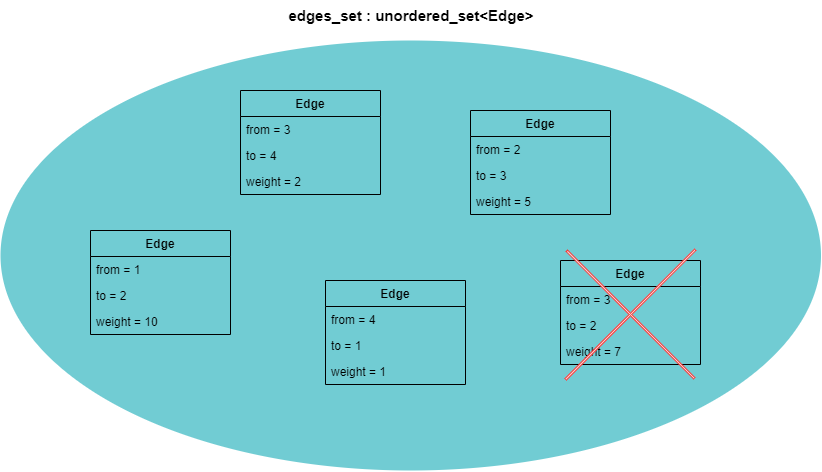
\includegraphics[width=0.7\textwidth]{./images/edges_setAbstract.png}
	\label{fig:edges_set}
\end{figure}

L'ultimo problema non ancora affrontato riguarda la possibilità di inserire un arco doppio tra due nodi uguali (come richiesto da problema), con la differenza che questi 2 archi hanno un peso diverso. Siccome la nostra implementazione non prevede la presenza di tali archi doppi, la funzione add\_eddge() si occupa di verificare l'eventuale presenza di un arco già inserito e di conseguenza i relativi pesi, per andare a modificare il peso qualora il peso del nuovo arco sia inferiore al peso dell'arco precedentemente già inserito. Per fare questo ad ogni aggiunta di un nuovo arco si va a verificare nella lista di adiacenza l'esistenza di un arco per quei due vertici:
\begin{itemize}
	\item \textbf{se l'arco era già stato aggiunto:} si confrontano i due pesi e si aggiorna il peso dell'arco solo nell'eventualità in cui il nuovo peso sia inferiore a quello già presente nella lista di adiacenza. Dopodiché se c'è stato un aggiornamento si aggiorna anche il relativo unordered\_set, eliminando l'arco precedente e si ri-aggiunge l'arco con il nuovo peso. 
	\item \textbf{se l'arco non era già stato inserito:} si inserisce l'arco sia nella lista di adiacenza che nell'unordered\_set.
\end{itemize}

Tutte le operazioni di aggiunta, per come sono implementati unordered\_set e unordered\_map in C++ hanno tempo costante e dunque l'operazione di aggiunta richiede tempo costante.


\subsubsection{Strutture Dati}

\subsubsection{Binary Heap}

\iffalse
The class that implements a Binary Heap data structure
can be instantiated as a MinHeap or a MaxHeap at compile-time. \\

We spared the \complexityN{} time required to build the heap at the beginning of Prim's algorithm because the \textit{std::vector} we use to initialize the list already respects the MinHeap property: the key related to the first element is 0, and every other key is $+\infty$. \\
\fi

\subsubsection{Priority Queue}

\subsubsection{Disjoint Set}

\subsection{Algoritmi}

\subsubsection {Costruzione del Grafo}
In questa parte si va a leggere il file di input per poi darlo in pasto alla funzione di costruzione della rappresentazione del grafo come spiegato nella sezione precedente.......

\subsubsection{Prim con Binary Heap}

\subsubsection{Kruskal Naive}
L'algoritmo Kruskal Naive è stato implementato a partire dallo pseudo codice visto in classe. A partire da questo ci si è subito accorti che una delle peculiarità di tale algoritmo e la necessità di verificare ad ogni inserimento di un arco di peso minimo la presenza di un ciclo nell'MST calcolato. Per ottenere tale funzionalità abbiamo deciso di modificare DFS in maniera da rilevare la presenza di un ciclo in un grafo. Per fare questo è stato creata la classe DFSCycleDetection, che è possibile ritrovare nella cartella "Shared", che data la rappresentazione del grafo e richiamando l'apposito metodo has\_cycle() è in grado di rilevare la presenza di un ciclo all'interno di esso usando per l'appunto una visita in profondità.\\

E' stato pertanto necessario modificare DFS nel seguente modo:
\begin{itemize}
	\item non è necessario avere una label per ogni arco che etichetti quell'arco come "DISCOVERY EDGE" o "BACK EDGE"
	\item quando un arco verrebbe etichettato come "BACK EDGE" nello pseudo codice visto in classe possiamo affermare che nel grafo è presente un ciclo. Non è necessario riscostruire tutto il ciclo come visto in un ulteriore modifica di DFS in classe.
	\item al posto di tener traccia di ogni arco se è stato visitato o meno attraverso l'attributo ID visto in clase, è stato deciso di creare un set di archi già visitati dove l'inseriemento e la ricerca avviene in tempo costante.
	\item per essere sicuri di non prendere in considerazione il vertice da cui viene lanciata ricorsivamente la DFS (ossia per non ritrovare il nodo da cui siamo venuti) è stata passata alla ricorsione il vertice padre, in modo che quando si scansiona la lista di adiacenza del vertice in considerazione non si consideri il vertice padre, simulando così il comportamento della funzione "opposite(v,e)" nel pseudo codice.
\end{itemize}

Per risolvere il problema di più di un eventuale componenente connessa nel grafo, vengono sempre scansionati tutti i nodi non ancora visitati attraverso un ciclo for su tutti i nodi come visto in classe.

Un ulteriore piccola ottimizzazione aggiunta è la verifica della presenza di soli 2 vertici in cui non è neccessario lanciare una visita in profondita, in quanto un ciclo non può sussistere tra 2 vertici se gli archi non sono diretti e non esistono self-loop TODO: VERIFICARE QUESTA SUPPOSIZIONE.

Un altra ulteriore ottimizzazione di tale algoritmo è la verifica ad ogni aggiunta di un nuovo arco che non crea un ciclo nel grafo, della soglia massima di archi che un MST può avere, che come visto in classe è pari al numero di nodi totali del grafo - 1. Pertanto non appena l'MST che si sta calcolando raggiunge la soglia prestabilità e possibile ritornare immediatamente l'MST.

Tale algoritmo risulta avere complessita dunque complessità O(mn) come visto in classe.


\subsubsection{Kruskal con Disjoint Set}
